In this chapter the website and it's functions are described. Furthermore, there will be some explanation about the logic that drives this website.

\section{Reason of it existence}
The website is the place where the online speakers and objects are manipulated.
The idea of the website was to enable the user to simply drag and drop speakers/objects with platform independency in mind.
The website had to be simple, easy to use and not dependent of some kind of webserver.
For this reason the website's main logic is made in JavaScript. The layout of this site was made with simple HTML and a small hint of CSS was used to bring it all up to flavor.

\section{Challenges}
- Loading settings
- MQTT with websockets
- syncronisation of the drawin area (still not 100\% reliable )

\section{Website layout}
In these following paragraphs, the layout and main usage of the site is explained.

\subsection{Idle}
In figure \ref{fig:website_idle} is the state of the website shown when it is in idle mode.
On the right hand side are the available speakers and objects. From here, the user can drag these in the draw area.

\begin{figure}[H]
    \centering
    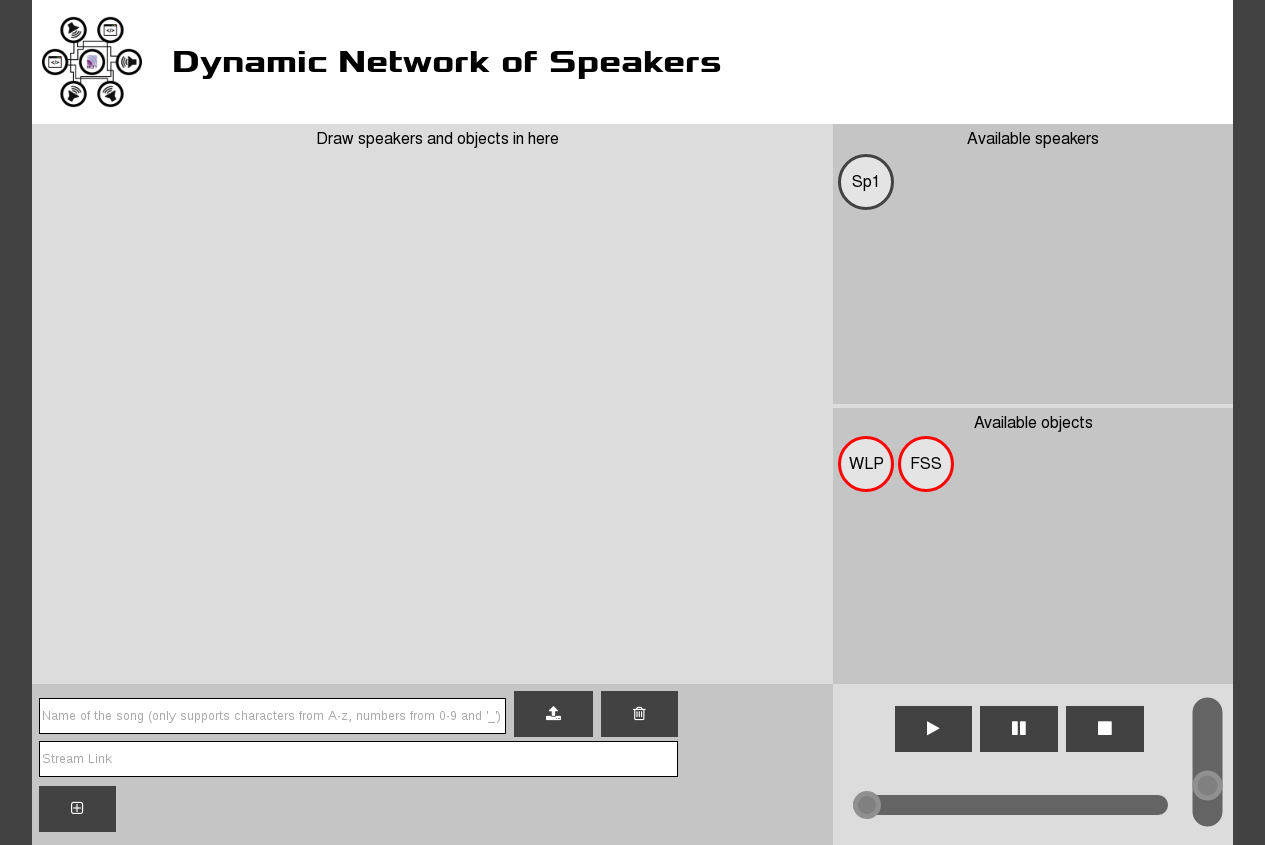
\includegraphics[width=.8\textwidth]{website_idle}
    \caption{Website when idle}
    \label{fig:website_idle}
\end{figure}

\subsection{Manipulating speakers and objects}

Demo of usage, one and two objects.
\begin{figure}[H]
    \centering
        \begin{minipage}[b]{0.5\textwidth}
            \centering
            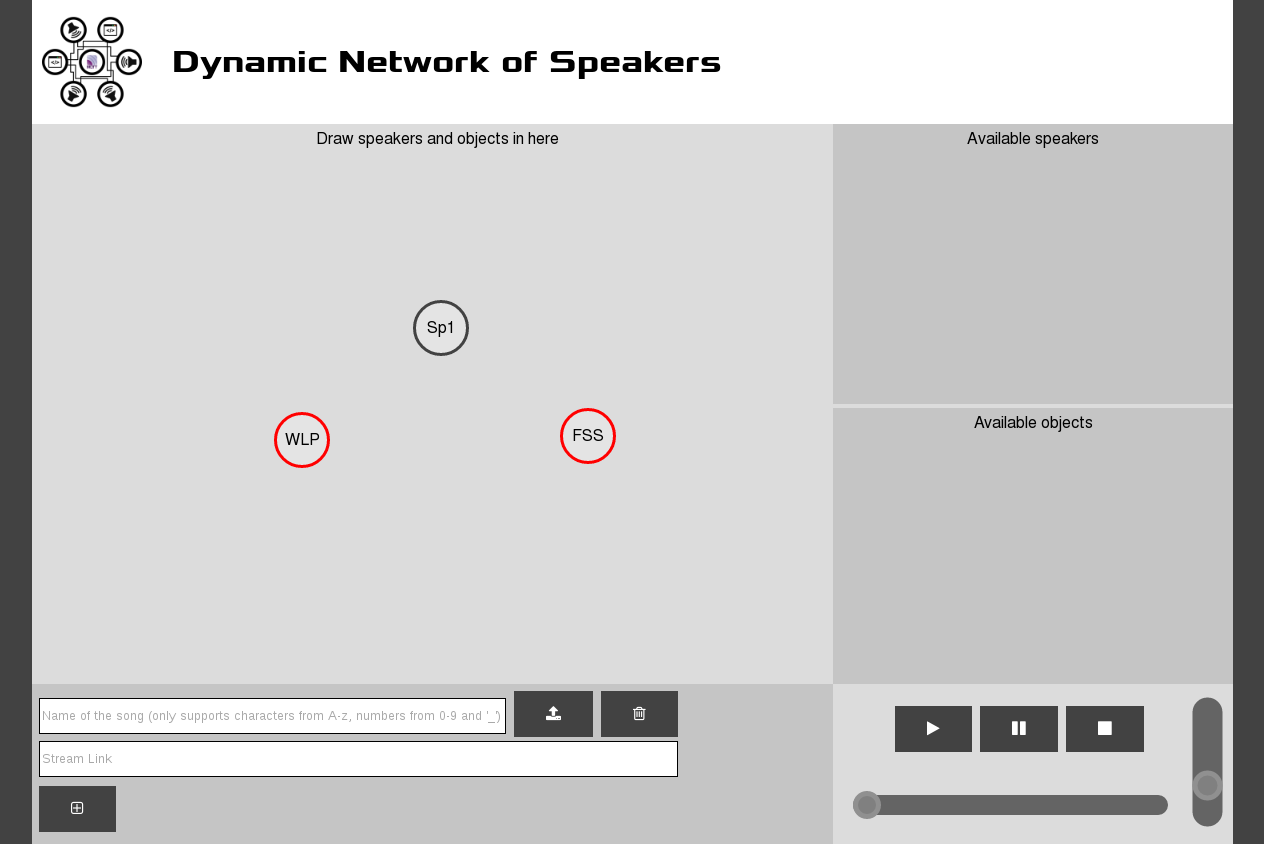
\includegraphics[width=.9\textwidth]{website_1sp_2obj}
            \caption{One speaker and two objects}
            \label{fig:website_1sp_2obj}
        \end{minipage}%
        %
        \begin{minipage}[b]{0.5\textwidth}
            \centering
            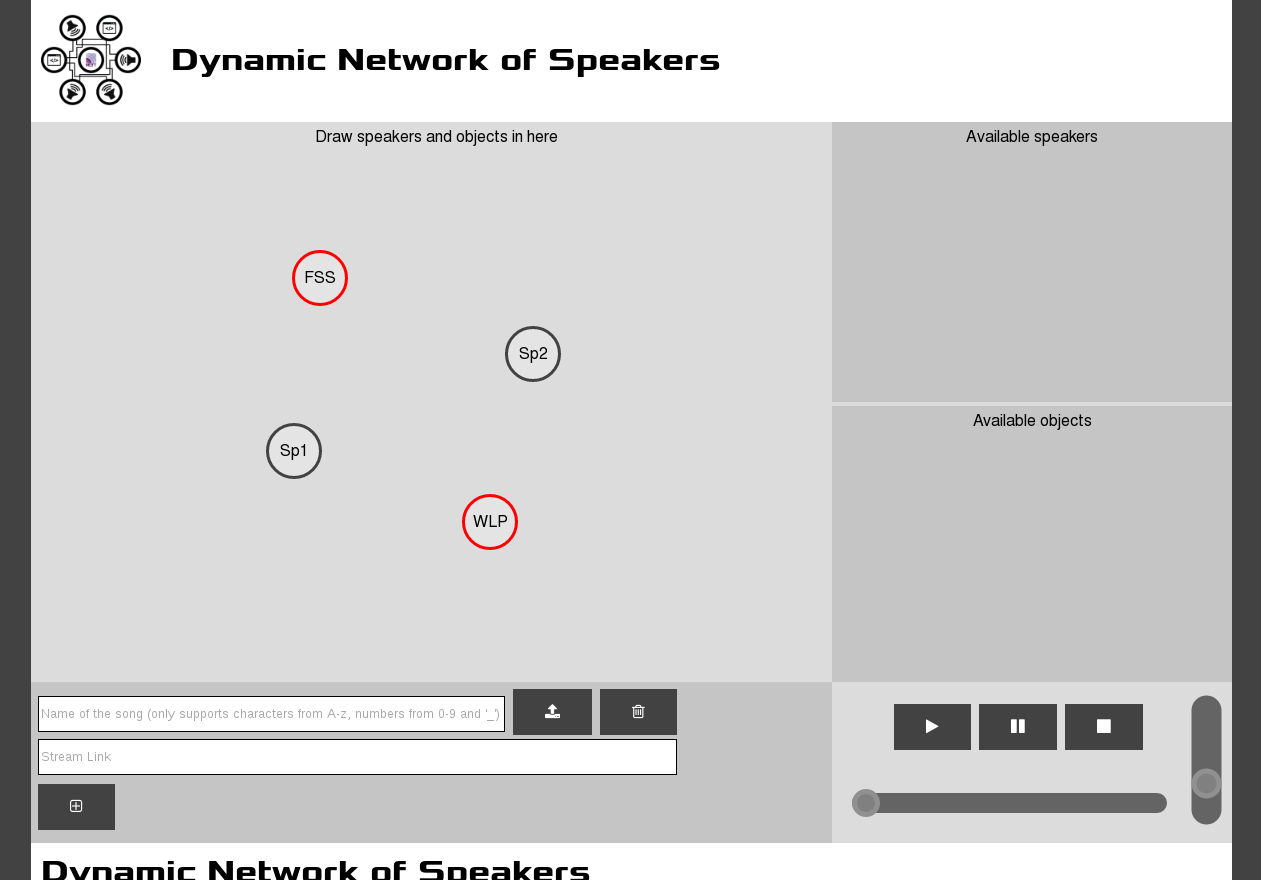
\includegraphics[width=.9\textwidth]{website_2sp_2obj}
            \caption{Two speakers and two objects}
            \label{fig:website_2sp_2obj}
    \end{minipage}
\end{figure}

\subsection{Edit objects}

Edit objects
\begin{figure}[H]
    \centering
    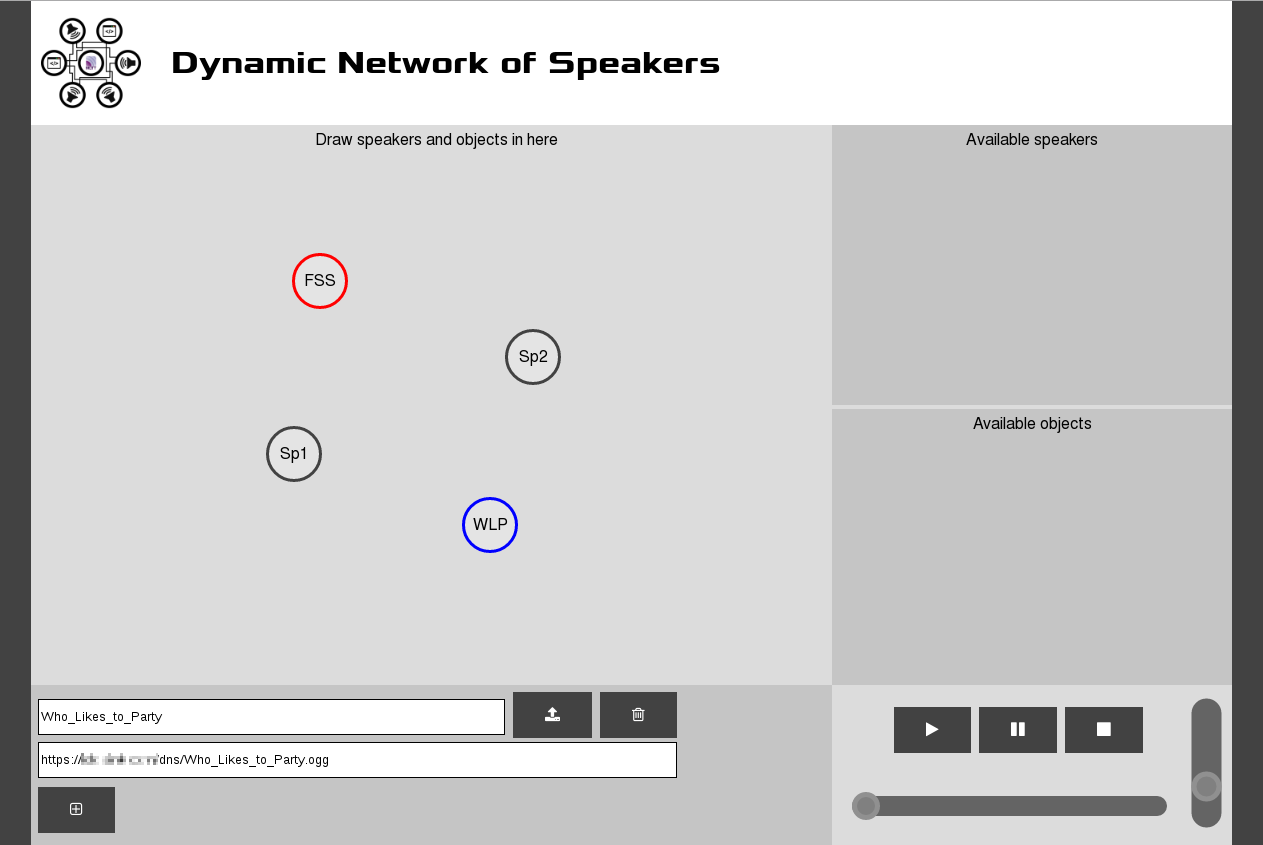
\includegraphics[width=.8\textwidth]{website_edit_object}
    \caption{Edit an object}
    \label{fig:website_edit_object}
\end{figure}

\subsection{Extra options}
Extra options

\begin{figure}[H]
    \centering
    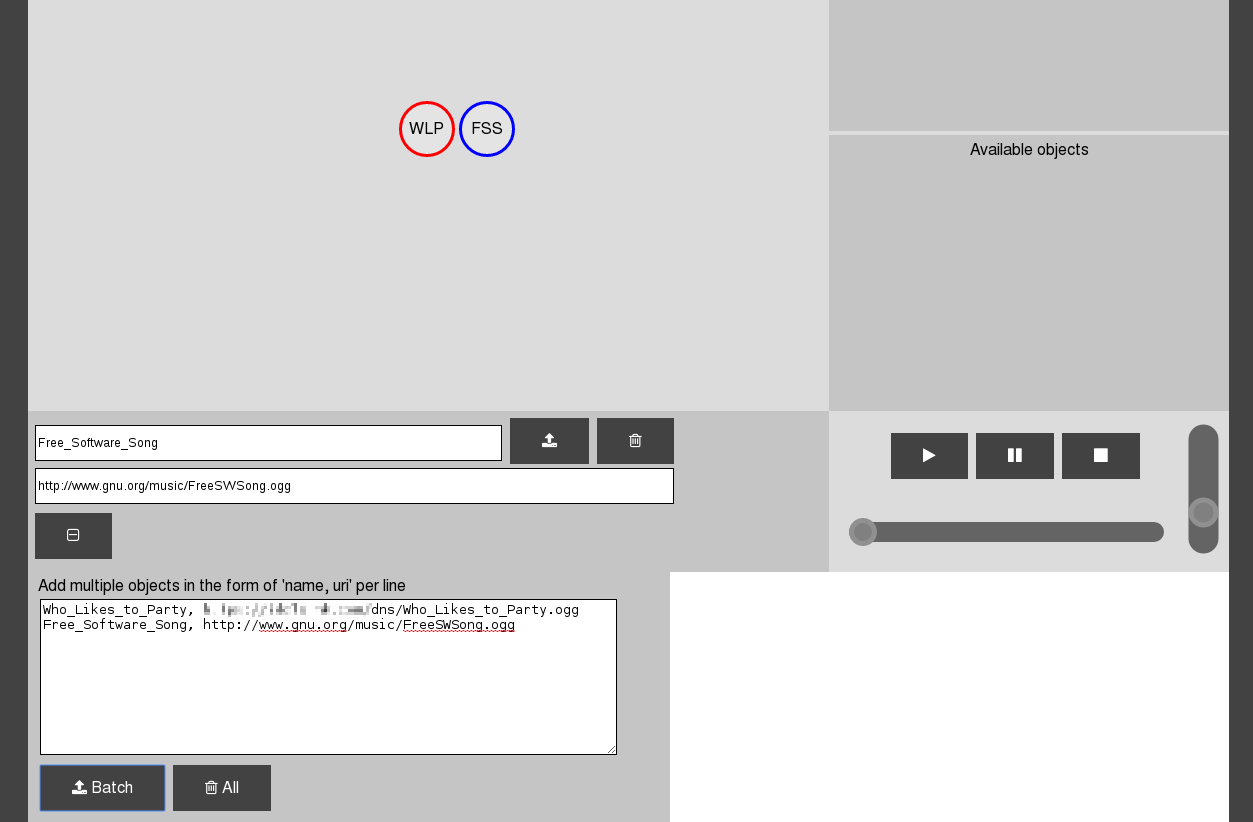
\includegraphics[width=.8\textwidth]{website_extra_options}
    \caption{Extra options}
    \label{fig:website_extra_options}
\end{figure}
